%!TEX root = ../../perdespassup.tex

\chapter[Persuasive Design for Password Support (P4P)]{Persuasive Design for Password Support}\label{chap:perdespassup}
Having reviewed the literature (Part \ref{part:related_work}), and explored both contextual factors (Part \ref{part:problem_space}) and novel designs (Part \ref{part:design_space}), we can now take a step back and synthesize common streams, results, and lessons learned. 
% GOAL: Support users in any kind of task that involves passwords. 
As a result, this chapter presents a new framework for researchers and designers to find and evaluate persuasive strategies that support users in any task that involves passwords. 
% Why is this necessary? / Motivation: covariates disregarded
We can find numerous research papers that evaluate a specific aspect without much context information or covariates. For instance, many types of password meters have been designed and evaluated, but most focused on measuring impact in the form of resulting password strength and usability metrics alone. However, aspects like user's preexisting mental models of password strength or the deployment environment were often untouched. At the same time, it is important to focus on the users and choose the support strategy that works best for them under a given configuration of environmental variables. 
% motivation: previous approaches might have lacked structure leading to lower efficacy 
Moreover, we find that many persuasive strategies stay below their potentials \cite{Renaud2017LessonsLearnedNudges}, or show unexpected effects (see Chapter \ref{chap:decoy}). Therefore, I establish a design process to avoid past shortcomings in nudging effects and to aid strategic decision-making for persuasive design. 


The \textbf{Persuasive Design for Password Support} (\textbf{P4P}) framework broadens the view on exploring and designing support systems (see Figure \ref{fig:p4p:passup}). It is divided into two ``lenses'' for the task. The ``research lens'' covers the ever-changing, heterogeneous environmental factors in usable password authentication and how to elicit them. It helps explain \textit{why} users act in certain ways and can provide pointers as to \textit{why} we should try to change the current state. The ``design lens'' assesses the status quo of password authentication and helps find solutions of different obtrusiveness levels (first stage), i.e. \textit{what} should be the focus of a new persuasive strategy. The second stage defines a user-centered process to implement once the required level of support has been decided. It aids in finding out \textit{how} the persuasive strategy should look. In the following, I explain these elements and show a design exercise where I apply the framework to create a novel approach for a password manager. 

%there won't be a formula like ``if X then use strategy Y'' (magic wand strategy). Rather, one needs to give different aspects some thought. 

%%%%%%%%%%%%%%%%%%%%%%%%%%%%%%%%%%%%%%%%
%
% FRAMEWORK FIGURE
%
%%%%%%%%%%%%%%%%%%%%%%%%%%%%%%%%%%%%%%%%
\begin{figure}[!htbp]
	\centering
	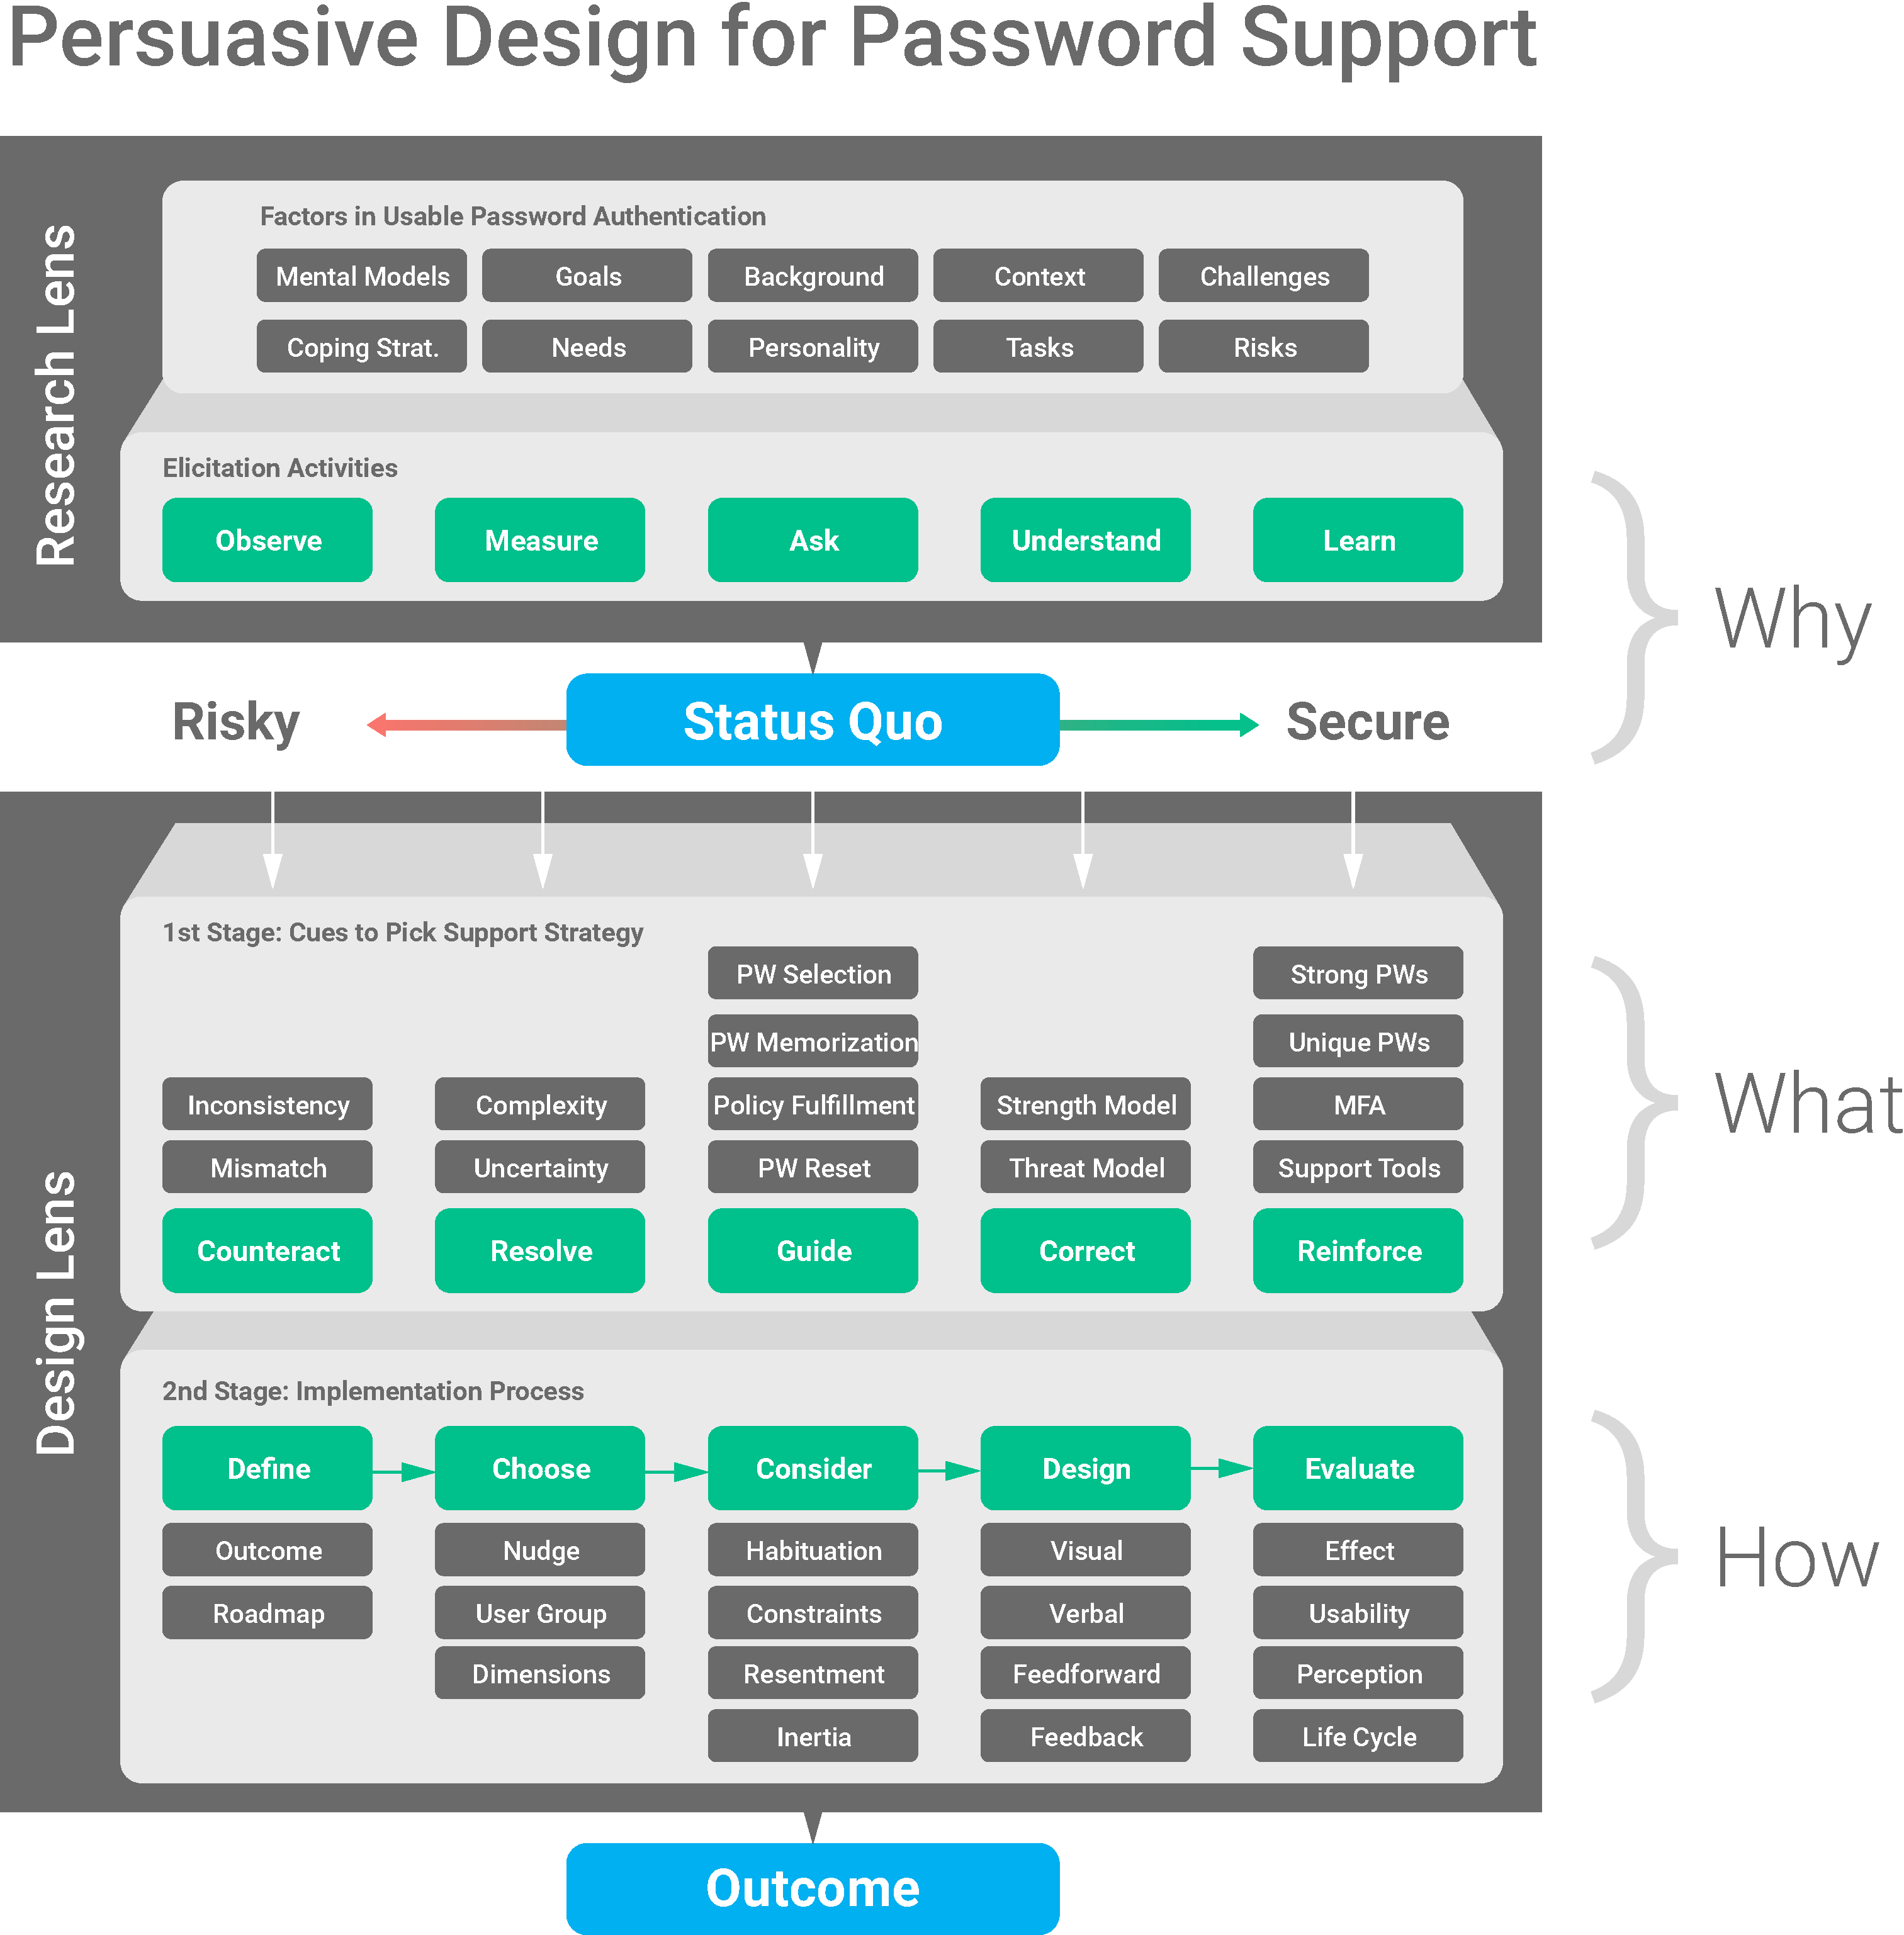
\includegraphics[width=\linewidth]{figures/pst/PerdesPassup}
	\caption{\label{fig:p4p:passup} Persuasive Design for Password Support (P4P) is a specialized design framework for strategic intervention development.}
\end{figure}

%%%%%%%%%%%%%%%%%%%%%%%%%%%%%%%%%%%%%%%%
%
% RESEARCH LENS
%
%%%%%%%%%%%%%%%%%%%%%%%%%%%%%%%%%%%%%%%%
\section{Research Lens}
% Assumptions -- reduce assumptions. 
The first step to create a novel persuasive support strategy is to elicit a number of factors that are involved in usable password authentication. Some of them have been addressed in previous research, e.g. coping strategies, while others are a direct consequence of the findings presented in this thesis (e.g. mental models or personality). 
% table
Researchers can try to answer the following questions to obtain an overview of the status quo of risky and secure factors:
%\begin{tabular}{p{14cm}l}

\vspace*{0.5cm}
\noindent
\resizebox{\linewidth}{!}{
\begin{tabular}{|p{14cm}l|}
	\hline
	\textbf{Question} & \textbf{P4P Element} \\
	What are current mental models, e.g. of password strength or support tools? & Mental Models\\
	How do different user groups cope with passwords? & Coping Strategies \\
	What are users primarily trying to achieve when they authenticate? & Goals \\
	What are the dimensions of user needs in this context, also in regard to support? & Needs \\
	How does demographic background impact password attitudes and behavior? & Background\\
	How much is personality visible in attitudes and behavior regarding authentication? & Personality \\
	What is the broader context of the authentication task, e.g. personal vs. work environment? & Context \\
	What (sub-)tasks does the user need to perform to reach their goals? & Tasks \\
	What are the challenges that different users face in the task? & Challenges \\
	What risks are there if the user acts insufficiently secure? & Risks\\\hline
\end{tabular}
}
\vspace*{0.5cm}

Some of these questions already hint at the dynamics of certain factors. For instance, users' mental models about threats might adapt over time, e.g. after falling prey to a phishing scam. Adoption rates of password managers are also volatile and the percentage of people relying on them certainly affects the type of novel support strategies one can implement. Although many questions and aspects can be answered by desk research methods, the dynamic evolution of the factors requires ongoing elicitation. Thus, traditional empirical research methods can be used to \textbf{observe} behavior and problems, \textbf{measure} interactions, explicitly \textbf{ask} users about certain aspects, \textbf{immerse} in the context of different user groups, and \textbf{learn} from all these activities. The result of this exploration is a detailed picture of the status quo. 

%%%%%%%%
% Questions
%%%%%%%
%\section{Guiding Support Strategies}

\subsubsection{Roadmap}
\begin{tabular}{p{14cm}l}
	What is the desired outcome? & Outcome \\
	How difficult is it to achieve and why? & Difficulty \\
	How big would the impact be? & Impact \\
	How important is it to achieve this outcome? & Importance
\end{tabular}

\subsubsection{Strategy}
\begin{tabular}{p{14cm}l}
	What exactly is the strategy based on? & Foundation\\
	Why is it expected to work? & Support\\
	What stage(s) in the password life cycle does it target? & Stage \\
	What is the specific context? & Context \\
	Are there other ways to achieve the same effect? & Alternatives \\
	Who is the target user group? & User Group\\
	How does the strategy relate to other frameworks? & Relationships\\
	Is it a one-off effort or continuous support? & Time-Scale \\
\end{tabular}

\subsubsection{Prerequisites}
\begin{tabular}{p{14cm}l}
	What are the dimensions of user needs in this context? & Needs \\
	How can the needs be met by the strategy? & Match \\
	What are the characteristics of the strategy? & Characteristics\\
	What are the minimum abilities that the user needs to have? & Abilities\\
\end{tabular}

\subsubsection{Risks}
\begin{tabular}{p{14cm}l}
	Will users get habituated to the strategy and is this good or bad? & Habituation\\
	How would the strategy interfere with other solutions? & Interference\\
	Does the strategy require too much effort from the users? & Effort\\
\end{tabular}

\subsubsection{Evaluation}
\begin{tabular}{p{14cm}l}
	How is the strategy going to be evaluated? & Method\\
	Is it possible to triangulate methods? & Triangulation\\
	What are the metrics to track impact? & Metrics	
\end{tabular}



\subsubsection{Status Quo}
% subjective assessment, but there are certain cues that
The status quo is a snapshot of the levels and relative importance of the factors that contribute to usable password authentication. Although the data elicitation should be generalizable and objective, the judgment of the result is not. It is up to researchers to collaboratively assess the risk level of a certain user group in various contexts. Here, the framework posits that some aspects that have traditionally been considered ``risky'' behavior need to be seen in a different light as attacks and countermeasures evolve. This follows the argumentation of Florêncio, Herley, Bonneau, and Van Oorshot among others \cite{Bonneau2012ReplacePasswords,Florencio2016CommACM, Herley2012PersistenceOfPasswords,ZhangKennedy2016RevisitingPasswordRules}. For instance, not all passwords need to withstand offline attacks. Therefore, it is unnecessary to nudge users to create passwords that would withstand them, because the usability drawbacks are unbearable for many users in most situations. The status quo thus informs the level of intervention in the subsequent design phase.

\section{Design Lens}
% pattern: If <user group> who <other factors | specific needs> do <cue>, then this can be seen as <risky|secure> and justifies <intervention>. 
The second half of the framework consist of two distinct stages: 1) Identifying the right level of support and 2) creating novel persuasive solutions. The first stage is strongly influenced by the results of the status-quo analysis, while the second deals with the specific questions during the implementation of a persuasive strategy. 

\subsubsection{Cues to Pick the Right Support Strategy} The interventions in Figure \ref{fig:p4p:passup} are ordered by their level of justifiable obtrusiveness. On the left, very risky behavior should be tried to \textbf{counteract}. The risk-level assessment is context dependent and can be read from the status quo analysis, where context is one dimension. We can read the elements like ``if X then Y'' in vertical direction. In particular, the framework follows this pattern:

\vspace*{1em}
\noindent
\fbox{
	\hspace{0.03\linewidth}
	\centering
	\parbox[c][2cm]{0.9\linewidth}{
		If \textit{<user group>}, who are \textit{<list of factors>}, do \textit{<specific action>}, then this can be seen as \textit{<risky or secure>} and justifies \textit{<intervention level>}.
	}
	\hspace{0.03\linewidth}
}
\vspace*{1em}

\noindent For example, the framework suggests that if \textit{users of online web-services} show \textit{clear patterns of inconsistent reuse}, i.e. reusing a password from a high-value account on a low-value website, then this is \textit{risky }behavior and should be \textbf{counteracted} with obtrusive strategies. The same goes for mismatches of account value and password strength. Other aspects can be \textbf{resolved} with less user-involvement and obtrusion. For instance, if status quo analysis shows that current password policies in companies are too complex, they should thus be replaced by simpler versions. Decisions under uncertainty, e.g. when a user needs to assess how valuable an account is, can be resolved with different persuasive patterns, too. Users can be \textbf{guided} in password selection, memorization, and reset tasks, as well as fulfilling a given policy. Moreover, it might be reasonable to \textbf{correct} users' mental models of password strength, respectively threats, to empower them to behave more consistently in the long term. Finally, there are a number of aspects that are generally beneficial in terms of security, e.g. using strong and unique passwords, activating multi-factor authentication (MFA), or relying on support tools like password managers. If these are part of the status quo for a given user group, there is no need to change that behavior for the time being. Rather, a support strategy should then positively \textbf{reinforce} these actions. 

\subsubsection{Implementation Process} Once the correct level of support has been identified, the P4P framework helps with implementing it. First, it is feasible to \textbf{define} the envisioned outcome of the strategy, e.g. ``stronger passwords'' or ``changing novices' mental models of password managers''. Moreover, the general context and roadmap for the implementations are defined at this point. Afterwards, the designer \textbf{chooses} a number of parameters for the strategies. Most notably, the nudging strategy to achieve the target outcome should be chosen and matched to the required level of user support. At the same time, the target user group should be narrowed down, e.g. with \glspl{persona} as shown in Section \ref{sec:personality:personas}. The different dimensions of user needs are already addressed at this stage, i.e. ``show'', ``explain'', ``help'', ``empower'', because they guide subsequent design stages. When the parameters have been fixed, it is important to \textbf{consider} a number of pitfalls in persuasion strategies. For instance, how quickly would users become \textit{habituated} to the nudge and how can one counteract that? What are the \textit{constraints} in different contexts, e.g. deploying the strategy at a company versus a consumer-oriented website for mobile devices? Users also often \textit{resent} attempts to be persuaded, thus the design needs to be more empathetic and ethical at the same time. Moreover, people prefer sticking to current behaviors although they theoretically want to act differently. This discrepancy results in a certain level of \textit{inertia} that a persuasive strategy needs to overcome to be effective. The list of considerations is not exhaustive but covers the most important aspects. If these limtations are too strong, it might be necessary to return to the previous step in the process to resolve them. 

Once there is reason to assume that the overall nudging strategy might be feasible, it needs to be substantiated with different \textbf{designs}. Here, password interventions have four degrees of freedom: \textit{visual} or \textit{verbal} nudges (e.g. in password meters), and feedforward or feedback techniques (e.g. password suggestions vs. strength assessment of the current password). It is important to consider different versions of the nudge in each of these dimensions to better exhaust the design space. Moreover, it allows for more nuanced options to \textbf{evaluate} the overall strategy. Typically, the \textit{effect} or impact of the nudge are compared to a control group, or between different configurations, e.g. the resulting password strength with various feedback mechanisms. The \textit{usability} and \textit{subjective perception} can be evaluated both quantitatively and qualitatively. Finally, it should be investigated how the nudge impacts the \textit{password life cycle} as a whole. 

\subsubsection{Outcome}
When the process has been completed in full, we are able to judge the feasibility of the strategy and may or may not recommend adopting it. If it is adopted, the status quo is likely to change after a given amount of time. This warrants exploring further opportunities and updating the factors in the ``research lens''. Thus, the framework needs to be seen as an iterative process, but it is flexible enough to take shortcuts and start at a later stage. In the following, I discuss an application of the P4P Framework to shed more light on its feasibility. 


%%%%%%%%
% DESIGN EXERCISE
%%%%%%%
\section{A Design Exercise with the P4P Framework}
Dealing with a multitude accounts, users mostly resort to password reuse. Although some reuse behavior involves considerable risk, Florêncio \etal indicated that it is a necessary strategy if users refrain from using password managers \cite{Florencio2014PasswordPortfoliosFiniteUser}. Consequently, Zhang-Kennedy \etal updated common recommendations on reuse  \cite{ZhangKennedy2016RevisitingPasswordRules}. In essence, they recommend to ``\textit{\textbf{strategically}} reuse passwords''. Moreover, Wash \etal stated that ``defining \textbf{appropriate categories} of websites for re-use of passwords of varying strengths is an open area of research;'' \cite{Wash2016UnderstandingPasswordChoices}. We used this as a starting point for a design exercise with the P4P framework. The section is partially based on a Bachelor thesis by Magdalena Siferlinger \cite{Siferlinger2017BAThesis} and a Master thesis by Martin Prinz \cite{Prinz2017Thesis}. I provided the ideas, supervised both students, and guided them through their projects.

\subsection{Phase 1: Research Lens}
The goal of the first phase to get a full picture of the status quo. This involves desk research, as well as empirical research methods. 

\subsubsection{Users: Mental models and Strategies}
One of the missing puzzle pieces are the specific categories that form reuse strategies. Although related work mentioned distinct exemplary categories, we wanted to narrow down the theoretical space. For this purpose, we planned and executed a mixed-method study to elicit re-use strategies. 35 people completed an online survey that was distributed on social networks. Five passers-by were interviewed in a public location in Munich. The questionnaire was identical in both methods, but the interviews allowed us to ask follow-up questions. Apart from demographics, we mainly inquired the number of accounts, password coping and reuse strategies, and the biggest challenges that respondents face in them. To elicit selection strategies, we provided four scenarios that involved creating accounts for email, social networking, banking, and a news page.

Unsurprisingly, most respondents reported that they reuse passwords either directly or with modifications (77.2\%). The remainder relied on a password manager to generate new random passwords. Mangling strategies were predictable (swapping letters for digits, varying appended symbols, and capitalizing letters). More importantly, a thematic analysis of the statements about reuse strategies revealed the following nine themes: Account type (e.g. email accounts), importance (e.g. very important, ``throw-away''), strength (e.g. one or two strong and a few weak passwords that are used depending on the perceived threat), time of creation (e.g. the year), frequency of reuse (e.g. a go-to password and a few less frequently typed ones), purpose (e.g. all accounts that were created for a project), base-password plus mangling algorithm, policy-driven (e.g. if the go-to password is rejected, a more complex password is reused), or generating completely new one depending on certain cues. These themes contribute to the status quo of password reuse in this design exercise.  
%Moreover, we found that participants relied on associations between the password and its purpose.  


\subsubsection{Password Managers} 
Other respondents mentioned using password managers, but there are different types of managers: they can be classified as either \textit{retrieval-based} or \textit{generative}. Retrieval-based password managers store the user's passwords securely and allow, e.g., to automatically fill out log-in forms on behalf of the user. Once a password is in the user's manager, they can choose to never type it again. Most commercial solutions work this way. On the downside, users do not ``practice'' their password as much and might not remember it in situations where the password manager is unavailable or too risky to use, e.g. at public computer at an airport. The generative password manager approach solves this problem, because no passwords are stored \cite{McCarney2012Tapas}: it provides the user with an algorithm to re-produce unique passwords (e.g. PwdHash\footurl{https://pwdhash.github.io/website/}{23.03.2018})  %Halderman \etal presented Password Multiplier that uses a master password and hash functions to generate unique passwords for different sites \cite{Halderman2005ConvenientPWM}. Users only need access to the Password Multiplier browser extension and their credentials to log in from any place. Chiasson \etal, however, found both usability and security problems with the system \cite{Chiasson2006PasswordManagers}. Maqbali and Mitchell later formalized this approach and sketched a new idea for pseudorandom passwords they called ``AutoPass''\cite{Maqbali2016PasswordGenerators}. It takes the master password, first part of the URL and optionally a digital object (e.g. a file, website, email address \cite{Biddle2011DigitalObjectsPWs}) to resolve some issues pointed out by Chiasson \etal. Stobert and Biddle developed another generative password manager called VersiPass, which is closely related to our approach \cite{Stobert2014PWMThatDoesntRemember}. It works similar to Password Multiplier, but is based on graphical authentication as master password (PCCP \cite{Chiasson2008PCCP}). Moreover, accounts are categorized by purpose.

%%%%%%%%%%%%%%
%
% 	COMPARISON
%
%%%%%%%%%%%%%%
% Table generated by Excel2LaTeX from sheet 'PWRM Benchmark'
\begin{table}[tbp]
  \centering
  \caption{\label{tbl:pwrm:pwm_comparison} Popular password managers: Comparison of features beyond password storage and retrieval. ✓ = available (✓) = available with restrictions, (✘) = with workaround, ✘ = not available}
  \resizebox{\linewidth}{!}{
  \begin{tabular}{rlllll}
	\multicolumn{1}{l}{\textbf{Category}} & \textbf{Feature} & \textbf{Dashlane} & \textbf{LastPass} & \textbf{1Password} & \textbf{KeePassX} \\
	\midrule
	\midrule
	\multicolumn{1}{l}{Automation} &       &       &       &       &  \\
	& form-detection & ✓     & ✓     & ✓     & (✘) \\
	& autofill passwords & ✓     & ✓     & ✓     & (✘) \\
	& autofill personal info & ✓ & ✓ & ✓ & ✘\\
	& autofill payment info & ✓ & ✓ & ✓ & ✘\\
	& facilitate password reset & (✓)   & (✓)   & ✘ & ✘\\
	& auto-update password reset & ✓ & (✓) & (✓) & ✘ \\
	\multicolumn{1}{l}{Organization} &       &       &       &       &  \\
	& grouping / tags / folders & ✓ & ✓ & ✓ & ✘\\
	& default groups & ✓ & ✘ & ✘ & ✘\\
	& memorization support & (✓)  & (✓) & (✓) & ✘ \\
	& password hints & (✓)   & ✘ & ✘ & ✓\\
	& cross device synchronization & ✓ & ✓ & ✓ & (✘)\\
	& personal info wallet & ✓ & ✓ & ✓ & ✘\\
	&       &       &       &       &  \\
	\multicolumn{1}{l}{Security Audit} &       &       &       &       &  \\
	& strength feedback (ad hoc / in client) & ✓ & ✓ & ✓ & ✘ \\
	& overall score & ✓ & ✓ & (✓) & ✘\\
	& ad hoc guidance & ✓ & ✓ & ✓ & ✘\\
	& security alert & ✓ & ✓ & ✓ & ✘ \\
	& negative feedback on reuse & ✓ & ✓ & ✘ & ✘\\
	& warn about inconsistent reuse & (✘)  & ✘ & ✘ & (✘) \\
	\multicolumn{1}{l}{Password Generation} &       &       &       &       &  \\
	& ad hoc random password & ✓ & ✓ & ✓ & ✓ \\
	& context aware (policy constraints) & ✘ & ✘ & ✘ & ✘ \\
	\multicolumn{1}{l}{Integrations} &       &       &       &       &  \\
	& Desktop  & ✓ & ✓ & ✓ & ✓\\
	& Browser & ✓ & ✓ & ✓ & (✓)\\
	& Smartphone & ✓ & ✓ & ✓ & (✓) \\
	\multicolumn{1}{l}{Collaboration} &       & (✓)   & ✓ & (✓)   & ✘ \\
	\multicolumn{1}{l}{Pricing} &       &       &       &       &  \\
	& Free Version & ✓ & ✓ & ✘ & ✓\\
	& Open Source & ✘ & ✘ & ✘ & ✓\\
\end{tabular}%  
}%end resizebox
\end{table}%


In Chapter \ref{chap:mental_models_pwm}, we have already presented an exploration of the mental models of password managers. The most important take-away was that only those who have started using one actually know the benefits, while non-users see password managers as a black box. In chapter \ref{chap:pws_and_personality}, we found that using a password manager was associated with demographic factors and some personality traits: Older participants and those with an IT background were more likely to rely on one, while people scoring high on ``openness'' were slightly less likely. To understand the status quo, we can compare real-world PWMs by their features (see Table \ref{tbl:pwrm:pwm_comparison}). Additional aspects were part of a recent coverage in the c't magazine\footurl{https://heise.de/-3992417}{22.03.2018}. 


%TODO maybe show how the elicitation was structured. (observe, measure, ask, understand, learn)
Relying on data from previous chapters, related work, and an additional small-scale empirical evaluation, we can frame the status quo like this:


\vspace*{1em}
\noindent
\fbox{
	\hspace{0.03\linewidth}
	\centering
	\parbox[c][13cm]{0.9\linewidth}{
		\subsubsection*{Status Quo of Password Reuse and Password Managers}
		% users need support, because:
		\textbf{Mental Models.} Users have very vague mental models about password managers. \textbf{Coping Strategies.} Although more people are starting to rely on password managers, the foremost coping strategy is reuse. Here, users often categorize accounts with varying granularity. We have identified nine distinct reuse strategies. \textbf{Goals.} Reusing facilitates recall. Some users are aware of the security risks of reuse and try to mitigate them by strategically reusing passwords. Current password managers try to steer users away from reuse altogether. \textbf{Needs.} Users need to be able to recall their most important passwords, while the rest could be handled by a password manager. \textbf{Background.} Older users appear to be more likely to reuse passwords, but also more willing to use a password manager. Having an IT background also often goes along with using PWMs to be able to handle a multitude of strong, more random passwords. \textbf{Context.} If users encounter PWMs at work, they are likely to continue using it in private. \textbf{Tasks.} Password managers can follow either a generative or a retrieval-based approach which differ in the tasks that the user has to complete. Retrieval-based managers require less cognitive effort. Strategically reusing passwords might include a deliberate strategy, but is more likely developed intuitively. \textbf{Challenges.} Users are challenged with picking the ``right'' password manager, switching from one manager to another, and learning how to use them best. Reuse does not challenge users strongly, but recalling the correct category is sometimes troublesome. \textbf{Risks.} Reusing a password too often increases the risk of the ``domino effect'' if one account is successfully attacked. Forgetting the master-password of a password manager, e.g. after a long period of inactivity, can lock users out of all their online accounts at once. 
	}
	\hspace{0.03\linewidth}
}
\vspace*{0.5em}

\subsection{Phase 2: Design Lens}
With the status quo as starting point, we put on the design lens and pick the focus areas in which to support users with password managers. Particularly, we identified that current PWMs try to ``fix the user'' by giving negative feedback on reused passwords in case they analyze all saved credentials and display a security score. Thus, there is an opportunity to ``fix the system'' and better support users in strategic reuse. Hence, our idea is a ``Password \textbf{Reuse} Manager'' (PWRM). 

\subsubsection{First Stage}
We can address the following cues to figure out \textit{what} to support: Inconsistent reuse should be \textbf{counteracted} by the PWRM, while consistent reuse is acceptable. The PWRM can offer default categories to \textbf{reduce} complexity and aid in the decision whether to reuse or generate a new password. If a new password is recommendable, the PWRM can \textbf{guide} selection, memorization, and policy fulfillment. If the users realize the benefits, this can \textbf{reinforce} their choice to adopt a password manager in the first place. It is evident that a password manager is capable of addressing multiple support strategies at once (counteract, resolve, guide, and reinforce), because it is able to interact with the user at multiple touch points of password authentication. At this point, changing the users' mental models is not the PWRMs responsibility, but it might happen along the way. 

\subsubsection{Second Stage}
In the second stage of the Design Lens, we try to create a concrete implementation of the support strategies. 
\paragraph{Define.} The envisioned outcome is a password manager that better represents the user's current coping strategies and therefore facilitates adoption. The design should be iteratively improved until all common coping strategies are supported (Roadmap). 

\paragraph{Choose.} We can choose nudges for each support strategy. Counteracting inconsistent reuse should be done fairly obtrusively, because this kind of behavior generates the greatest risk, respectively the highest amount of effort in recovering from an attack. The ``commitment and consistency'' principle by Cialdini is perhaps the most promising candidate \cite{Cialdini2007Influence}. Resolving uncertainty and complexity can be addressed with \textit{suggestive} nudges, that facilitate decision-making. The ``salience'' effect falls into this category \cite{Coventry2014SCENEBehavioralNudges}. Also, having good \textit{default} categories is a powerful nudge \cite{Cranor2008FrameworkReasoning}. Similarly, users can be guided by simplifying the password selection process (simplification principle \cite{Forget2007PersuasionEducationSecurity}). Finally, using a password manager can be reinforced by offering the service for free and providing a good user experience overall. 

In our case, we target users who prefer reusing passwords but also appreciate help in this task. Thus, the target user group consists of novices who have developed their own reuse strategies and prefer maintaining these, but in a simpler way. The ``Eliot Elis'' persona from Chapter \ref{chap:pws_and_personality} represents this user group well. Therefore, the strategy should fulfill the ``show'' and ``help'' dimensions of user needs: Showing problems with inconsistencies and helping with finding alternatives are the foremost requirements we can address with the PWRM. At the same time, the PWRM should \textit{empower} users to maintain their strategy, and to decide not to store certain passwords but only the user-names or a hint. 

\paragraph{Consider.}
If the users stick to the PWRM, habituation is actually beneficial, because they learn how to leverage the tool to work for them. In terms of constraints, the PWRM is a piece of software that would need to pass security audits in company environments. Giving a lot of feedback and interventions might be perceived as authoritative and thus users could resent these strategies. At the same time, the mere presence of the above mentioned nudges might not overcome inertia, so the efficacy needs to be evaluated in multiple steps. 

\paragraph{Design.} 
In the design phase, we iteratively flesh out the specific information architecture and visuals of the PWRM. In multiple design sessions and evaluations we moved from a paper prototype to clickable wireframes, to a working prototype in the form of a browser extension. Figure \ref{fig:pwrm:conceptfinal} shows the central page of the PWRM browser extension. The user can put passwords into categories that share the same password. During onboarding, a few default categories based on past reuse strategies are automatically created. They user may also decide to save only a hint for a specific category (see Figure \ref{fig:pwrm:hintboxes}). This aims to avoid that the user worries about the security of the PWRM -- they can simply put the accounts that they do not want managed into one category. In that case, the PWRM still supports them by helping them recall the password, because the category acts as a hint. 

\begin{figure}[htbp]
	\centering
	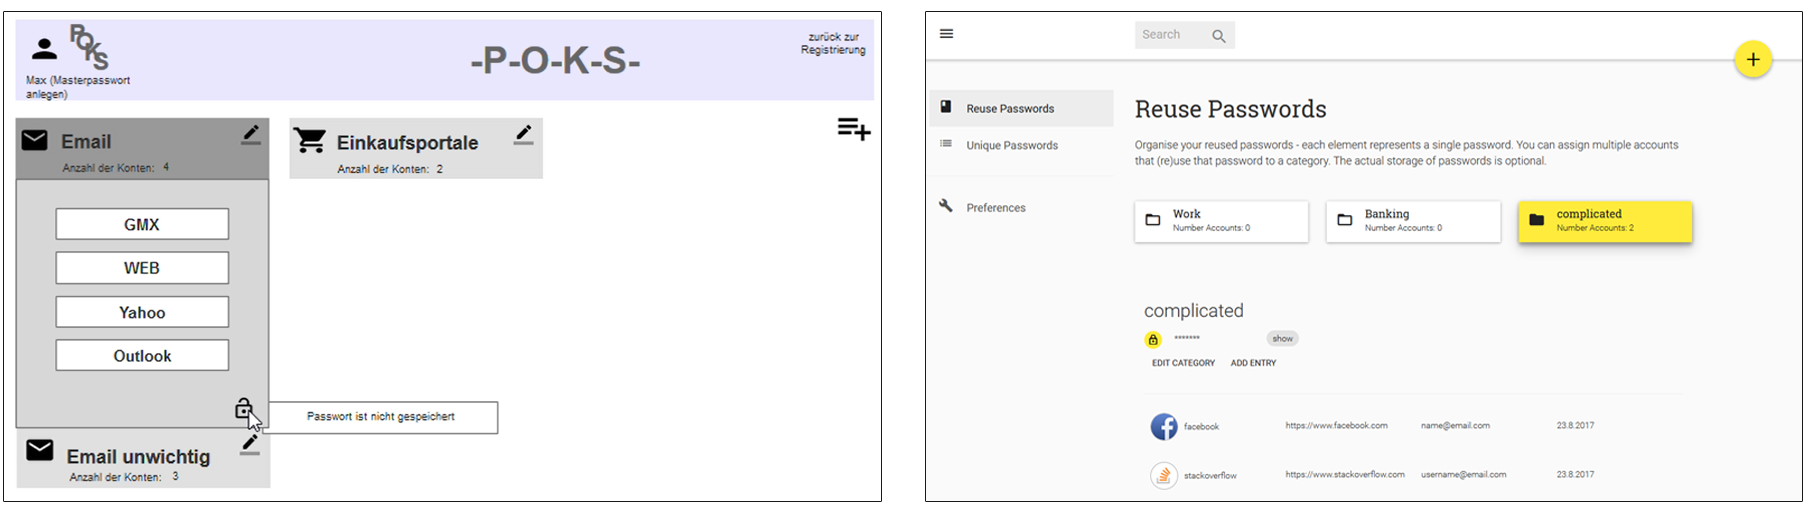
\includegraphics[width=\linewidth]{figures/pwrm/concept_final}
	\caption{Different stages of the design iterations. Left: wireframing stage. Right: The main page of the PWRM groups reused passwords into different categories, which makes it easy to indicate that a password has been reused too often. Nudges: \textbf{simplification} (through organization), \textbf{defaults} (default categories during onboarding)}
	\label{fig:pwrm:conceptfinal}
\end{figure}

\begin{figure}[htbp]
	\centering
	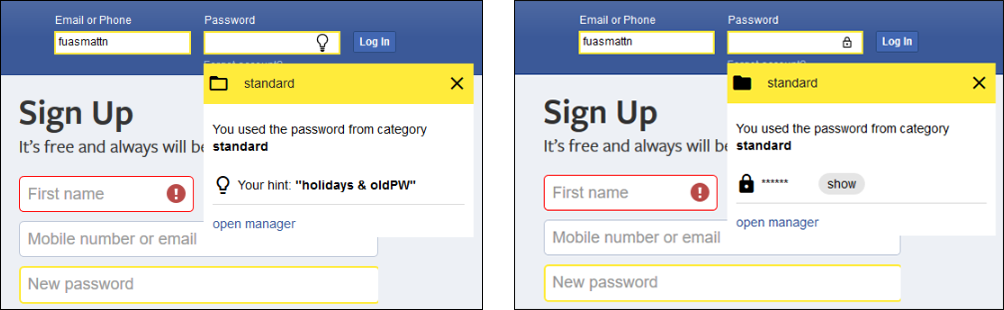
\includegraphics[width=\linewidth]{figures/pwrm/hintboxes}
	\caption{The PWRM mitigates trust issues by allowing the user to store password hints or categories instead of the passwords themselves. Nudges: \textbf{consistency} (stay within the category), \textbf{salience} (suggesting categories, visual framing)}
	\label{fig:pwrm:hintboxes}
\end{figure}

It is also possible to flag passwords as ``unique'', i.e. that they do not belong to a group of accounts that share the same password. Figure \ref{fig:pwrm:entry-unique} shows the page that also visually indicates the strength of the passwords. The PWRM browser extension detects ``submit'' events from forms that contain password fields. It opens a small pop-up window to let the user store the password (see Figure \ref{fig:pwrm:extension-popus}). Here, they can decide whether it should be put into one of the reuse-categories or become a ``unique'' password, that is not shared with other accounts. Further features and design decisions are indicated in the captions of Figures \ref{fig:pwrm:conceptfinal}, \ref{fig:pwrm:hintboxes}, \ref{fig:pwrm:entry-unique}, and \ref{fig:pwrm:extension-popus}.

\begin{figure}[htbp]
	\centering
	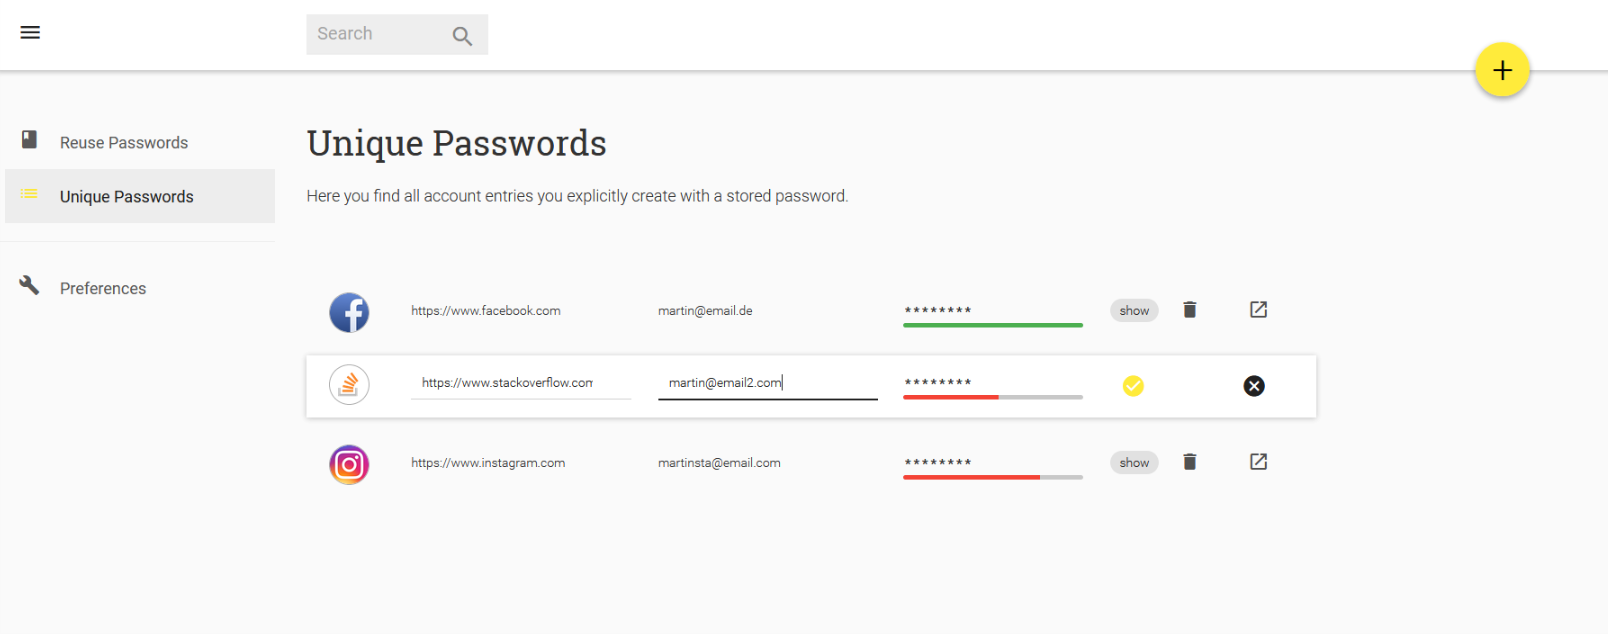
\includegraphics[width=\linewidth]{figures/pwrm/entry-unique}
	\caption{The PWRM holds a separate page of unique passwords. For the user, this reduces uncertainty about the security state of different accounts. Nudges: \textbf{commitment} (user should not reuse these passwords.)}
	\label{fig:pwrm:entry-unique}
\end{figure}
\begin{figure}[htbp]
	\centering
	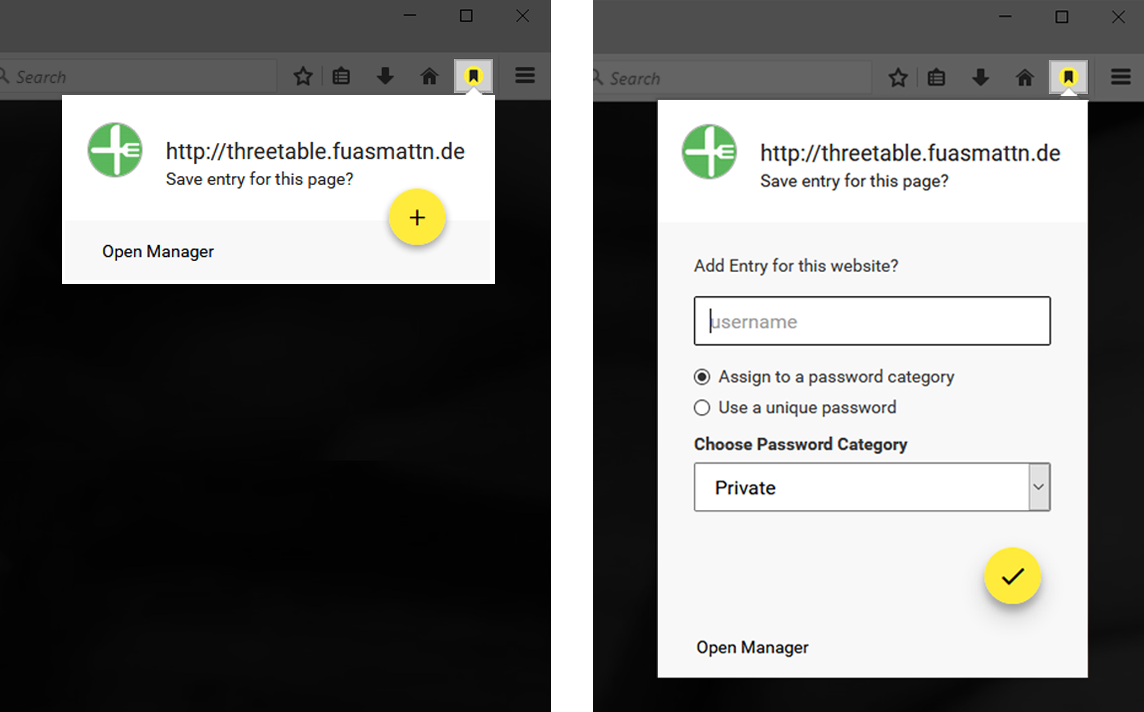
\includegraphics[width=0.9\linewidth]{figures/pwrm/extension-popus}
	\caption{The PWRM browser extension allows the user to save passwords to different categories. Nudges: Defaults, simplification}
	\label{fig:pwrm:extension-popus}
\end{figure}


\paragraph{Evaluate.} 
We iteratively evaluated the concept and the design in a user-centered approach. Table \ref{tab:pwrm:evaluations} shows the four evaluation methods at different stages of the process. In a first wizard-of-oz study, participants found that the categorization feature of the paper prototype was still too complex, although they liked the idea of grouping accounts by passwords. In the second evaluation, the need for more explanation about the potential risks of password reuse became evident. The first usability test with a preliminary implementation of the browser extension showed that participants were able to fulfill all tasks. However, they desired more automation features to speed up the interactions. Finally, we created a beta version of the PWRM extension and recruited 12 participants to test it for ten days. After the ten days, it was clear that the participants only rarely opened the browser with the extension, so we could not conclusively evaluate the solution. The qualitative feedback indicated that participants were browsing the web on their mobiles and also used other browsers during that time. Hence, as a caveat, the effects of the nudges and the impact on the password life cycle would only become visible in a longitudinal, large-scale study, with more careful screening. Unfortunately, this was outside of the scope of this design exercise, and we need to leave this to future work. 

\begin{table}
	\begin{tabular}{llrp{9cm}}
		\textbf{Stage} & \textbf{Focus} & \textbf{N} (m/f) & \textbf{Key Result}\\ \hline
		Paper Prototype & Concept & 5 (4/1) & Clarify categorization feature \\
		Clickable Wireframes & Information architecture & 7 (5/2) & Explain reuse risks \\
		Usability Test & Task success, problems & 6 (4/2) & Provide more, automated support \\
		Field Study & Usage patterns & 12 (6/6) & Smoother integration necessary
	\end{tabular}
	\caption{\label{tab:pwrm:evaluations} Evaluation iterations of the concept. }
\end{table}

\section{Summary}
This chapter contributes ``P4P'' - a framework for persuasive design for password support. Its elements are based on numerous research studies both from related and original work. Other persuasion frameworks for authentication, e.g. the Persuasive Authentication Framework \cite{Forget2007PersuasionEducationSecurity}, focused on the design space, whereas P4P tries to structure the investigation of the problem (the \textit{why}), design-heuristics (the \textit{what}), and the implementation process (the \textit{how}). So, although it might be seen as an approach to provide a ``holistic'' view on password support design, I intentionally avoided this term. The elements exhaust much of the research and design space, but there might be other latent factors or different configurations that need more attention in future explorations. Nevertheless, depending on the amount of status-quo information, the structure of the framework allows researchers and designers to start at a later point and follow a structured process. I showed how to use the P4P framework to tackle research questions and explore new opportunities in password support: It led to the creation of a ``Password Reuse Manager'' that is now under an open-source license to facilitate distributed development\footurl{https://github.com/mimuc/pwrm/}{23.03.2018}. The design exercise was fairly comprehensive and encompassed a multitude of strategies. However, the framework is also applicable for smaller tasks, e.g. the design of password meters. In the future, P4P can help derive novel solutions outside the current design space of password support. 

\vspace*{1.5cm}
\noindent
\fbox{
	\hspace{1cm}
	\parbox[c][7cm]{0.7\linewidth}{
		\section*{Take Aways}
		\begin{itemize}[leftmargin=*]
			\item The Persuasive Design for Password Support (P4P) framework structures exploration and design of new solutions to support users in any password-related task.
			\item It can be applied to big design projects (like a full-blown password manager in our case), but also to smaller aspects (like the design of password meters, help pages, onboarding wizards etc.)
		\end{itemize}
	}
	\hspace{1cm}
}

